\begin{figure*}
\centering
\scalebox{0.8}{
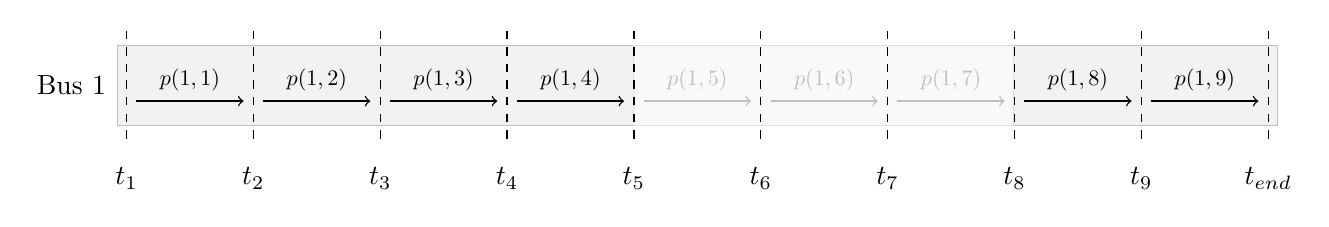
\begin{tikzpicture}
	\node[rectangle, draw=gray!50, fill=gray!10, minimum width=5.8in, minimum height=0.4in](bus1Box) at (7.75,0.8){};
	\node(bus1BoxLabel) at (-0.2, 0.8){Bus 1}; 
	\node[rectangle, draw=gray!25, fill=gray!5, minimum width=1.9in, minimum height=0.4in](bus1Box) at (7.75 + 1.6,0.8){};
	
	\foreach \curLab/\preLab[count=\c, evaluate=\c as \pos using {0.5 + (\c - 1)*14.5/9}] in {t_1/t_1, t_2/t_1, t_3/t_2, t_4/t_3, t_5/t_4, t_6/t_5, t_7/t_6, t_8/t_7, t_9/t_8, t_{end}/t_9}
	{
		\node[label=below:$\curLab$](b\c) at (\pos, 0){};
		\node(t) at (\pos, 1.4){};
		\ifnum\c>1 
			\node(b1Curr) at (\pos, 0.8 - 0.2){};
				\ifnum\c > 5
					\ifnum\c < 9 
						\def\clr{black!25}
					\else
						\def\clr{black}
					\fi
				\else
					\def\clr{black}
				\fi
				\draw[->, line width=0.5pt, \clr] (b1Prev.east) -- node[midway, above]{\scalebox{0.8}{$p(1,\number\numexpr\c-1)$}}(b1Curr.west); 
		\fi
		\node(b1Prev) at (\pos, 0.8 - 0.2){};
		\draw[dashed, line width=0.5pt] (b\c.north) -- (t.north); 
	}
	\path (b9.south) -- node[midway, below=0.1in]{$\hdots$}(b10.south);

\end{tikzpicture}}
\caption{Bus schedule with availability}
\label{fig:busAvail}
\end{figure*}

